\chapter{A main chapter}
\label{chap:firstchap}
\begin{figure*}
    \centering
    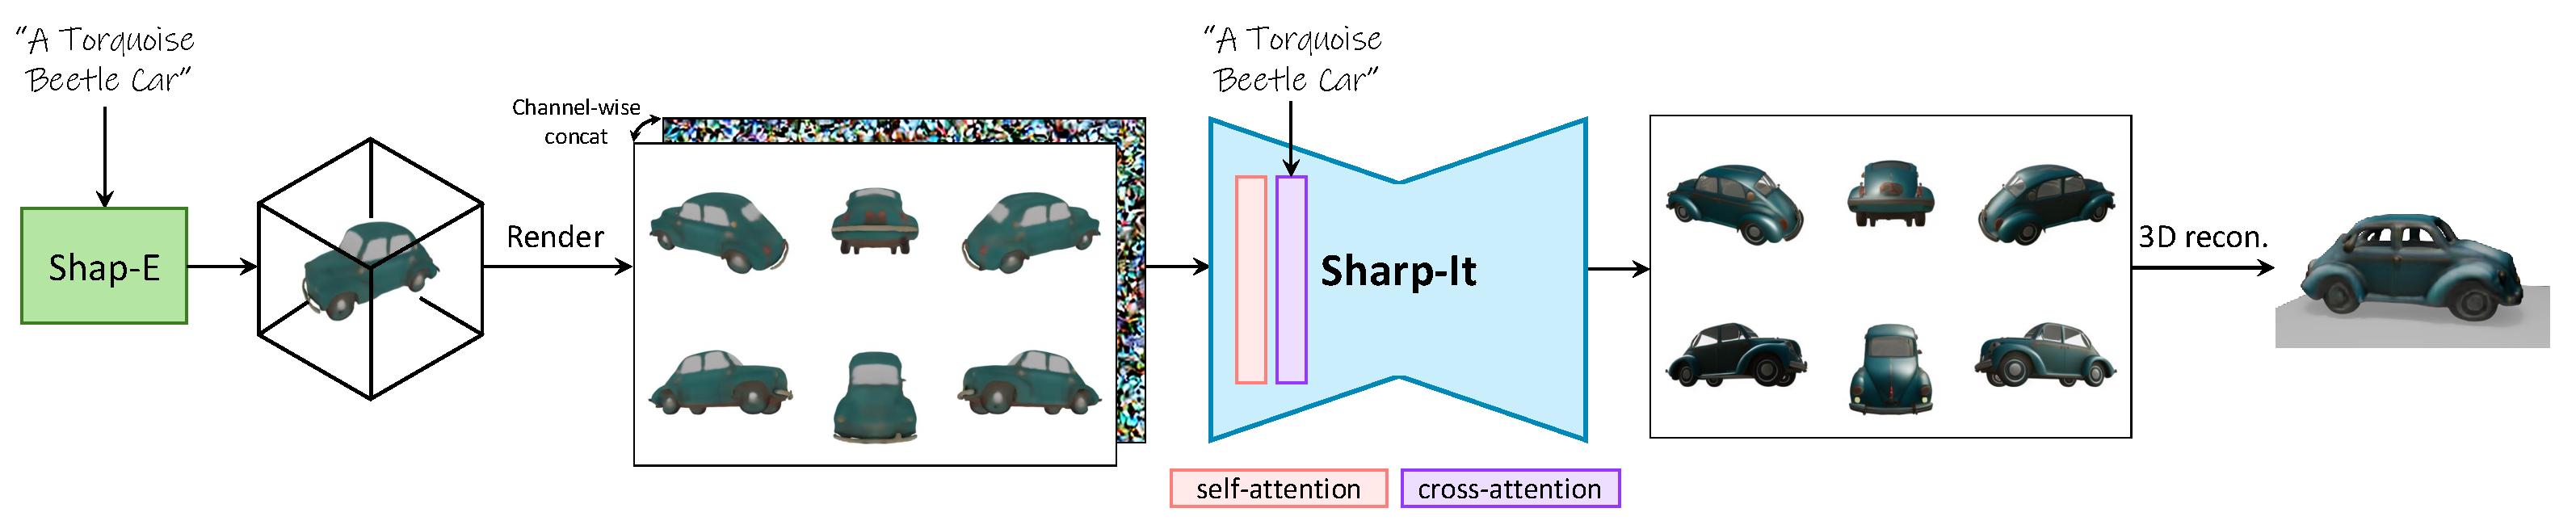
\includegraphics[width=\linewidth]{images/method_sharpe_new.pdf}
    \vspace{-18pt}
    \caption{Overview of 3D generation pipeline with Sharp-It.
    First, a 3D object is generated with Shap-E. Then, we render six views of this low-quality object. Sharp-It is a diffusion model based on Stable Diffusion~\cite{rombach2022highresolutionimagesynthesislatent} that enhances these views with the guidance of a text prompt by refining geometry and adding detailed appearance. Sharp-It employs cross-attention layers for text-based guidance and self-attention layers for cross-view consistency. A high-quality 3D object can be reconstructed from the multi-view image set.}
    \vspace{-12pt}
    \label{fig:method}
\end{figure*}
\section{Method}
In this section, we present our approach to addressing the quality gap between direct 3D generative models and those that reconstruct 3D objects from multi-view images.
We focus on Shap-E~\cite{jun2023shape}, a 3D generative model, and introduce \emph{\ourname}, a multi-view-to-multi-view diffusion model that enhances 3D objects generated by Shap-E. We train \ourname{} to improve these objects by adding intricate appearance details and correcting geometric artifacts such as discontinuities and broken parts.
% We begin by providing the necessary background on Shap-E and Zero123++, the diffusion models upon which \ourname{} builds.
The process of generating a 3D model with \ourname{} is demonstrated in Figure~\ref{fig:method}.

\subsection{Preliminaries}

\paragraph{Shap-E} 
is a latent diffusion model specifically designed for generating 3D assets. As common in latent diffusion models~\cite{rombach2022highresolutionimagesynthesislatent}, Shap-E is trained in two stages. In the first stage, an encoder is trained to map 3D objects into a latent space. This latent space corresponds to the weight space of implicit functions that represent 3D shapes, with each shape represented as an element in $\mathbb{R}^{1024\times1024}$. The latent representation can be decoded using Signed Texture Field (STF) rendering, where it is treated as the weights of an implicit function.
In the second stage, a diffusion model is trained within the Shap-E latent space, allowing for conditioning on either text or images.

\paragraph{Zero123++}
is an image-conditioned diffusion model designed to generate 3D-consistent multi-view images from a single input view~\cite{shi2023zero123singleimageconsistent}
. It builds upon Stable Diffusion~\cite{rombach2022highresolutionimagesynthesislatent}, which is a latent diffusion model comprising a VAE and a UNet. The VAE encodes images into a resolution that is eight times smaller and consists of four channels, while the UNet serves as the diffusion model, operating on the four-channel latent codes.
Zero123++ is a fine-tuned version of Stable Diffusion that accepts an image as input. Given an input image, it produces a $3\times2$ grid of $320\times320$ pixel images, with six constant azimuth and elevation angles. 
Originally, Zero123++~\cite{shi2023zero123singleimageconsistent} was designed to generate this grid image with a grey background. In InstantMesh~\cite{xu2024instantmesh}, it was further fine-tuned to render a white background, addressing the issue of ``floaties''—particles floating through space during 2D-to-3D lifting.

\subsection{Dataset Construction} \label{sec:data}
We begin by constructing a paired dataset consisting of degraded Shap-E objects along with corresponding high-quality objects. Our key idea in constructing the dataset is that such pairs can be obtained by employing the encoder of Shap-E in conjunction with a high-quality 3D objects dataset.
Specifically, we utilize objects from Objaverse~\cite{deitke2023objaversexluniverse10m3d}, provided by~\cite{luo2023scalable, luo2024view}, and encode them using Shap-E's encoder. For each pair of an object from Objaverse and its encoded Shap-E latent code, we render a $3\times2$ grid from six predefined camera views, applying three HDR lighting conditions. Our experiments, detailed in the ablation studies, indicate that rendering each object under varying HDR lighting enhances the model’s performance.

We apply a filtering criteria on the resulting dataset.
We remove objects where the degraded Shap-E rendering is significantly different from the original object's rendering, indicating a failure of Shap-E's encoder. Additionally, we filter out objects that are too thin or do not match certain keywords based on their annotated captions. For each remaining object, we extract a caption using BLIP2~\cite{li2023blip2}.
Finally, we split the dataset into training and test sets, resulting in 180,000 objects for training and 6,000 for testing.


\subsection{\ourname}
\ourname{} is a multi-view to multi-view diffusion model designed to enhance low-quality multi-view images of 3D objects generated by Shap-E. It takes as input a set of multi-view images rendered from a low-quality 3D object, along with a textual prompt, and produces high-quality multi-view images with refined geometric details and textures that correspond to the input views.
% In practice, the multi-view image set is organized as a grid of $3\times2$ views, resulting in a total resolution of $960\times640$. Each view has its own azimuth and elevation angles, which remain fixed across different objects. 
An overview of a 3D generation pipeline with \ourname{} is shown in Figure~\ref{fig:method}.

\paragraph{Architecture}
The architecture of \ourname{} has two key requirements: generating multi-view image sets and incorporating input multi-view sets as conditions. We build on Zero123++~\cite{shi2023zero123singleimageconsistent, xu2024instantmesh}, which was fine-tuned for multi-view generation, where images are arranged in a $3\times2$ grid with a total resolution of $960\times640$ and fixed camera angles across objects.
%
To enable multi-view conditioning, we modify the architecture of Zero123++ by expanding the UNet input to 8 channels: 4 for latent noise and 4 for the VAE-encoded Shap-E multi-view images. This design lets our model leverage the coarse geometry from the input views to achieve better 3D consistency, and is inspired by image editing techniques that fine-tune diffusion models to accept an image as input and modify specific parts while preserving others~\cite{brooks2022instructpix2pix, rombach2022highresolutionimagesynthesislatent, yang2022paint}. Unlike these approaches, which operate on a single image, our model learns to enhance the input views in a 3D consistent manner. 
Furthermore, we replace Zero123++'s image embedding with text prompts in the cross-attention layers, enabling better enhancement control and appearance editing capabilities (Section~\ref{sec:app-edit}).


The model we build on consists of self-attention layers, which play an important role in facilitating the consistency of our produced multi-view set~\cite{shi2024mvdream, wang2023imagedream}. Since our model operates on a multi-view image grid, these layers can be seen as an application of cross-view attention between the different views. Similarly to previous works~\cite{wang2023imagedream, shi2024mvdream, shi2023zero123singleimageconsistent}, this allows our model to simultaneously refine corresponding points across different views by learning the correspondences between them. 
We visualize the learned correspondences in Figure~\ref{fig:cross-view-attention}. The figure displays self-attention maps for a query point marked by a red dot in the leftmost image. The results demonstrate that this point on the wheel receives the highest attention weight across different views. Additionally, the attention mechanism identifies semantically similar points -- notably, other wheels of the car.

\begin{figure*}[t]
  %--- zero-width box that is shifted slightly left ---%
  \makebox[0pt][l]{\hspace*{\shift}%

    %------------- actual content -------------%
    \setlength{\tabcolsep}{3pt}
    \scriptsize
    \begin{tabular}{ccccccccc}
        & Input (Shap-E) & GaussianDreamer & MVEdit & MVDream w/ &
          Zero123++ w/ & Zero123++ w/ & Zero123++ w/ & Ours (Sharp-It)\\
        &                &                &         & SDEdit &
          SDEdit (U) & SDEdit (C) & SDEdit (R) \\[2pt]

        % avocado couch ---------------------------------------------------- %
        \raisebox{43pt}{\multirow{2}{*}{%
          \rotlabel{``An avocado shaped\\leather couch''}}} &
        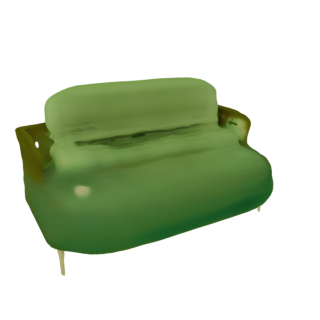
\includegraphics[width=\imgW]{images/comparison_plot/avocado_couch/shap-e/avocado_couch_view1_shap_e.png} &
        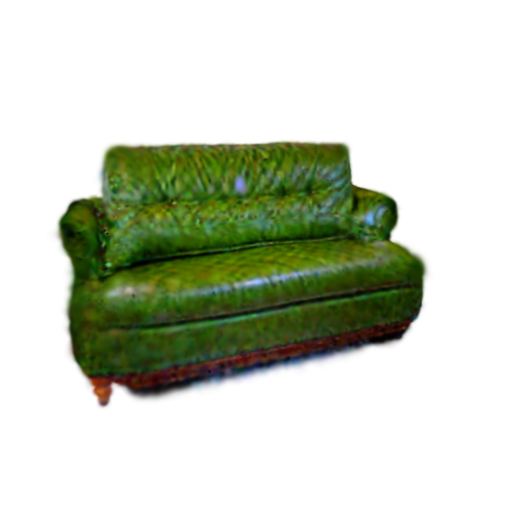
\includegraphics[width=\imgW,trim=30 30 30 30,clip]{images/comparison_plot/avocado_couch/gaussian_dreamer/1.png} &
        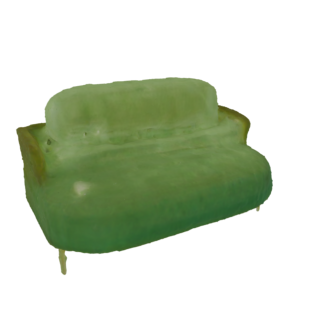
\includegraphics[width=\imgW]{images/comparison_plot/avocado_couch/mvedit/1.png} &
        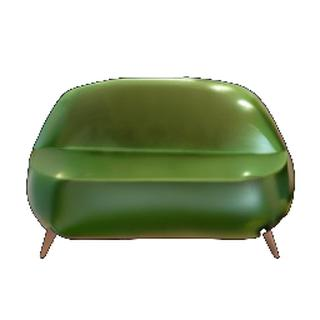
\includegraphics[width=\imgW]{images/comparison_plot/avocado_couch/mvdream/avo_couch_upscaled_3.jpg} &
        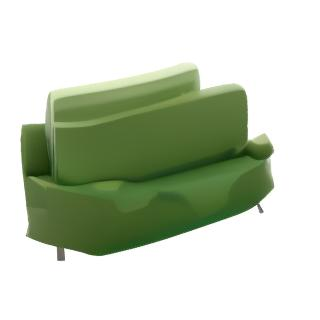
\includegraphics[width=\imgW]{images/comparison_plot/avocado_couch/zero123++/avo_couch_tile_2_3.jpg} &
        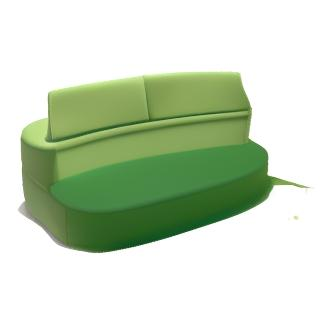
\includegraphics[width=\imgW]{images/comparison_plot/avocado_couch/zero123++image/avo_couch_tile_1_3.jpg} &
        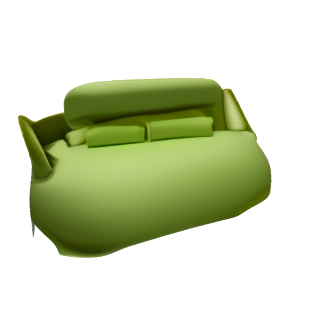
\includegraphics[width=\imgW]{images/comparison_plot/avocado_couch/zero123++refiner/split_image_0_2.png} &
        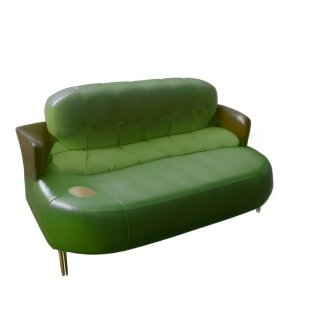
\includegraphics[width=\imgW]{images/comparison_plot/avocado_couch/sharp-e/avocado_couch_view1_sharp_e.png} \\

        & % second couch row
        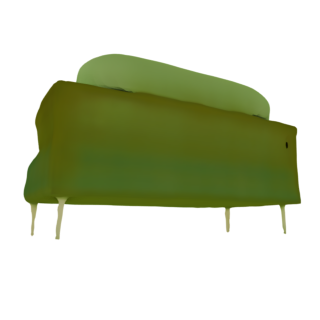
\includegraphics[width=\imgW]{images/comparison_plot/avocado_couch/shap-e/avocado_couch_view2_shap_e.png} &
        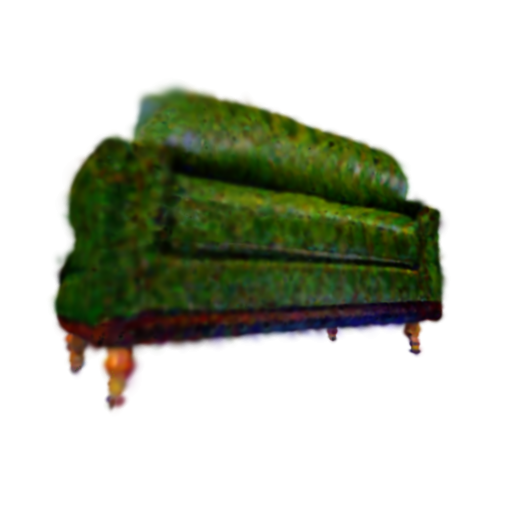
\includegraphics[width=\imgW,trim=30 30 30 30,clip]{images/comparison_plot/avocado_couch/gaussian_dreamer/3.png} &
        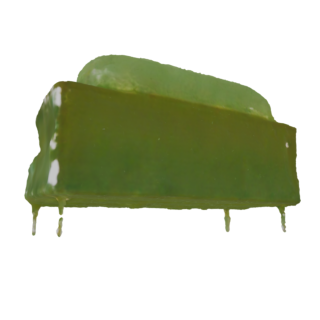
\includegraphics[width=\imgW]{images/comparison_plot/avocado_couch/mvedit/2.png} &
        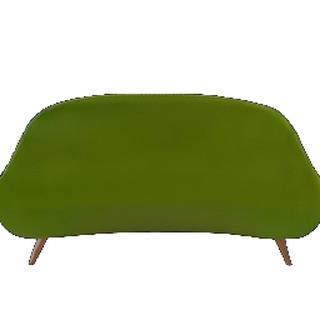
\includegraphics[width=\imgW]{images/comparison_plot/avocado_couch/mvdream/avo_couch_upscaled_1.jpg} &
        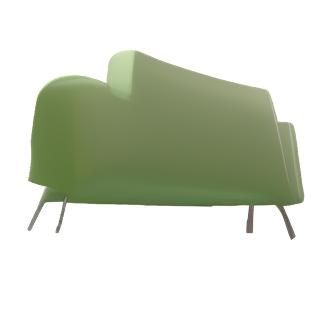
\includegraphics[width=\imgW]{images/comparison_plot/avocado_couch/zero123++/avo_couch_tile_2_6.jpg} &
        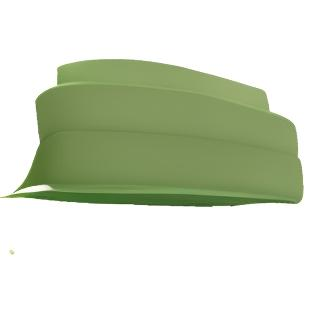
\includegraphics[width=\imgW]{images/comparison_plot/avocado_couch/zero123++image/avo_couch_tile_1_6.jpg} &
        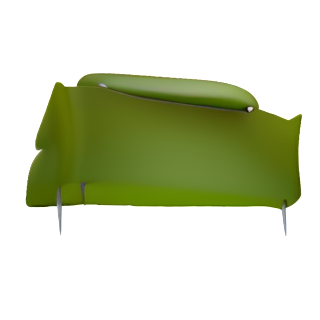
\includegraphics[width=\imgW]{images/comparison_plot/avocado_couch/zero123++refiner/split_image_0_5.png} &
        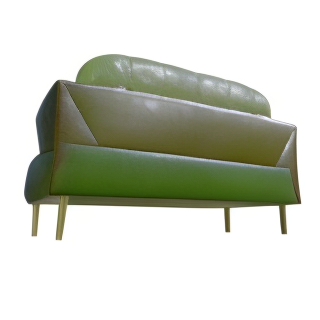
\includegraphics[width=\imgW]{images/comparison_plot/avocado_couch/sharp-e/avocado_couch_view2_sharp_e.png} \\[2pt]

        % bust -------------------------------------------------------------- %
        \raisebox{36pt}{\multirow{2}{*}{%
          \rotlabel{``A bust of a man\\with a beard''}}} &
        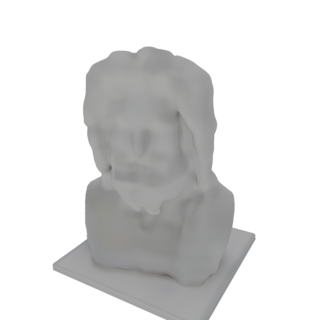
\includegraphics[width=\imgW]{images/comparison_plot/bust/shap-e/tile_0.png} &
        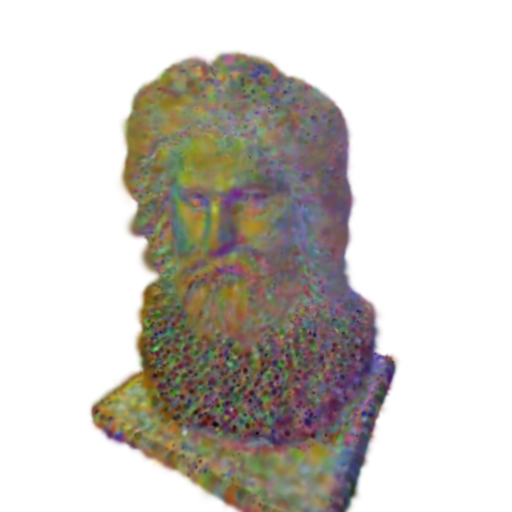
\includegraphics[width=\imgW]{images/comparison_plot/bust/gaussian_dreamer/0.png} &
        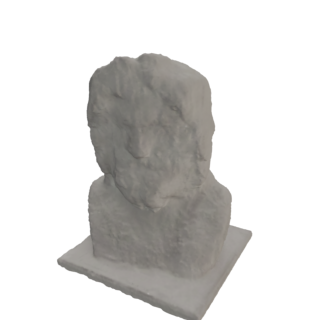
\includegraphics[width=\imgW]{images/comparison_plot/bust/mvedit/1.png} &
        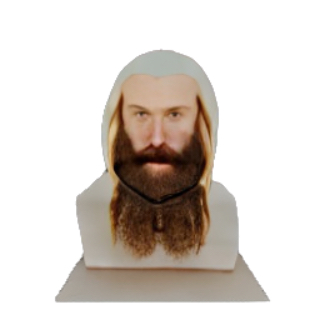
\includegraphics[width=\imgW]{images/comparison_plot/bust/mvdream/white_tile1.jpg} &
        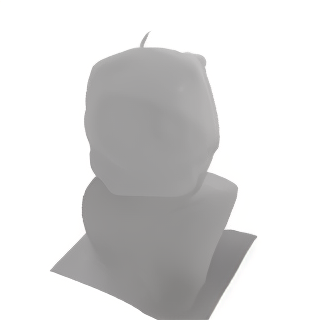
\includegraphics[width=\imgW]{images/comparison_plot/bust/zero123++/efbb32609fd44a4f849015e875bc57a1_tile_1.png} &
        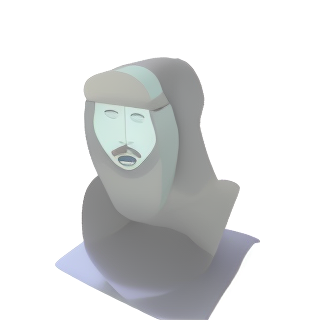
\includegraphics[width=\imgW]{images/comparison_plot/bust/zero123++img/efbb32609fd44a4f849015e875bc57a1_tile_1.png} &
        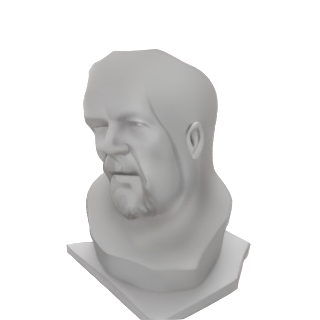
\includegraphics[width=\imgW]{images/comparison_plot/bust/zero123++refiner/split_image_1_0.png} &
        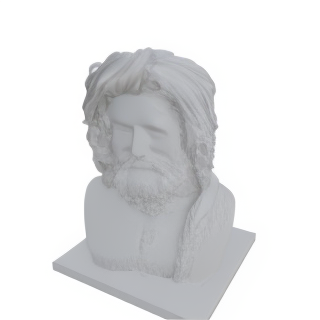
\includegraphics[width=\imgW]{images/comparison_plot/bust/sharp-e/efbb32609fd44a4f849015e875bc57a1_tile_1.png} \\

        & % second bust row
        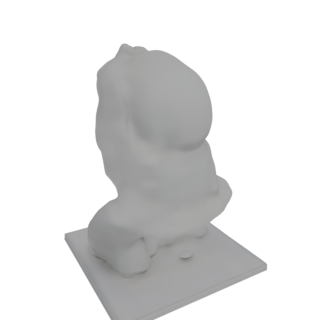
\includegraphics[width=\imgW]{images/comparison_plot/bust/shap-e/tile_2.png} &
        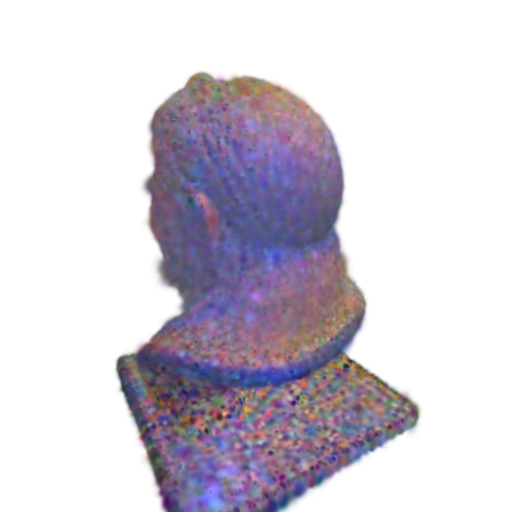
\includegraphics[width=\imgW]{images/comparison_plot/bust/gaussian_dreamer/bust_gaussian_dreamer_2.png} &
        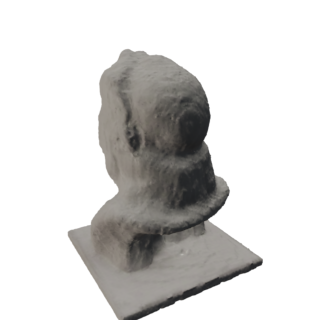
\includegraphics[width=\imgW]{images/comparison_plot/bust/mvedit/2.png} &
        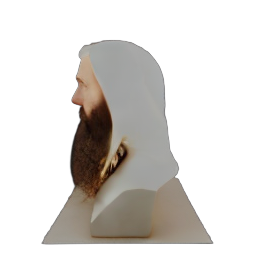
\includegraphics[width=\imgW]{images/comparison_plot/bust/mvdream/white_tile2.png} &
        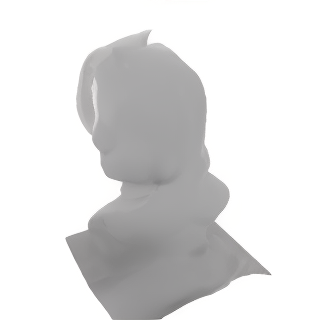
\includegraphics[width=\imgW]{images/comparison_plot/bust/zero123++/efbb32609fd44a4f849015e875bc57a1_tile_3.png} &
        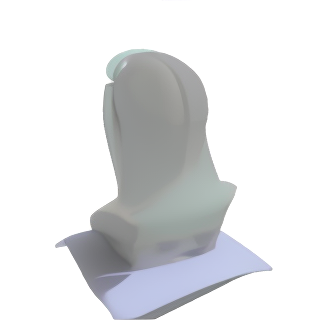
\includegraphics[width=\imgW]{images/comparison_plot/bust/zero123++img/efbb32609fd44a4f849015e875bc57a1_tile_3.png} &
        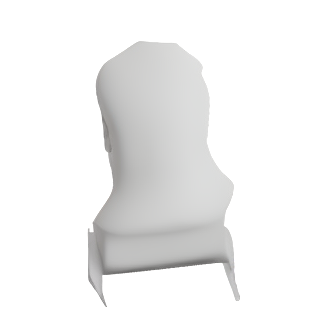
\includegraphics[width=\imgW]{images/comparison_plot/bust/zero123++refiner/split_image_1_2.png} &
        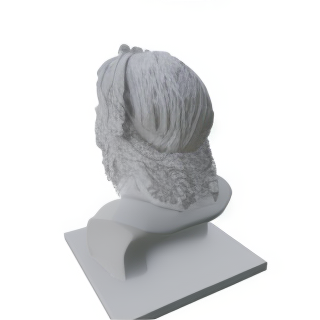
\includegraphics[width=\imgW]{images/comparison_plot/bust/sharp-e/efbb32609fd44a4f849015e875bc57a1_tile_3.png} \\[2pt]

        % tiki mask --------------------------------------------------------- %
        \raisebox{25pt}{\multirow{2}{*}{%
          \rotlabel{``A wooden\\tiki mask''}}} &
        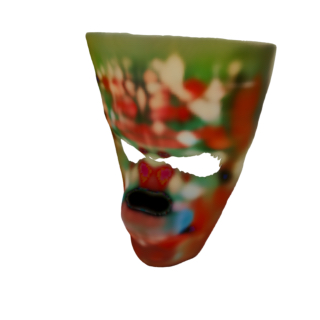
\includegraphics[width=\imgW]{images/comparison_plot/tiki_mask/shap-e/render_0000-4.jpg} &
        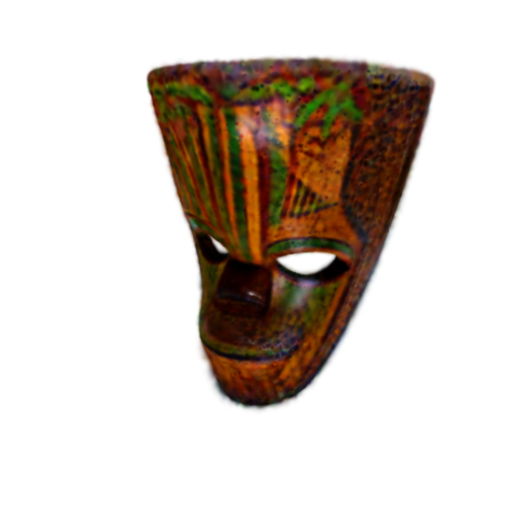
\includegraphics[width=\imgW]{images/comparison_plot/tiki_mask/gaussiandreamer/0.png} &
        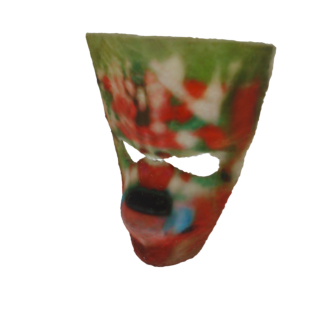
\includegraphics[width=\imgW]{images/comparison_plot/tiki_mask/mvedit/render_0000-3.jpg} &
        
\includegraphics[width=\imgW]{images/comparison_plot/tiki_mask/mvdream/tile_0.jpg} &
        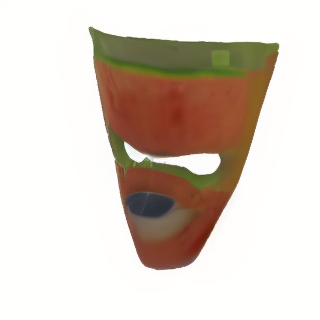
\includegraphics[width=\imgW]{images/comparison_plot/tiki_mask/zero123++unguided/avocado_couch_sdedit_steps_batch_0_tile_0.png} &
        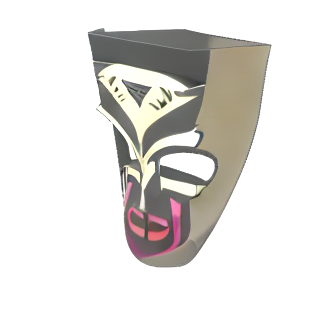
\includegraphics[width=\imgW]{images/comparison_plot/tiki_mask/zero123++guided/tiki_mask_guided_tile_0.png} &
        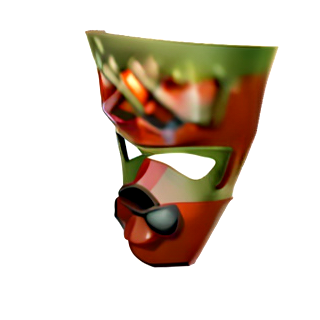
\includegraphics[width=\imgW]{images/comparison_plot/tiki_mask/zero123++refiner/split_image_2_0.png} &
        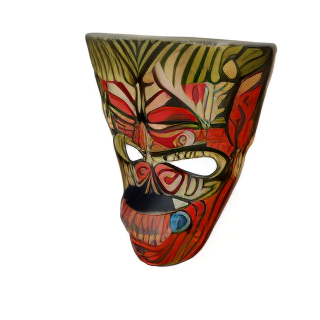
\includegraphics[width=\imgW]{images/comparison_plot/tiki_mask/sharp-e/10_75_steps_batch_0_a_wooden_tiki_mask_tile_0.png} \\

        & % second tiki row
        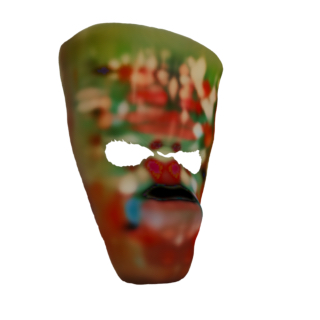
\includegraphics[width=\imgW]{images/comparison_plot/tiki_mask/shap-e/render_0005-2.jpg} &
        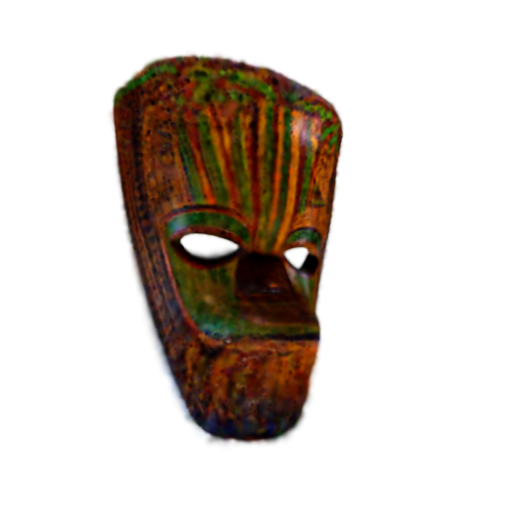
\includegraphics[width=\imgW]{images/comparison_plot/tiki_mask/gaussiandreamer/3.png} &
        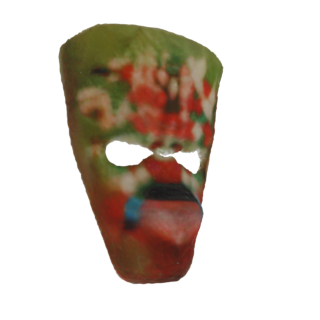
\includegraphics[width=\imgW]{images/comparison_plot/tiki_mask/mvedit/render_0005.jpg} &
        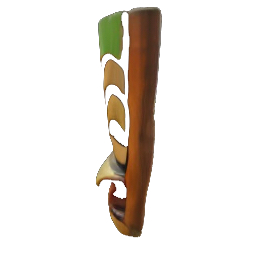
\includegraphics[width=\imgW]{images/comparison_plot/tiki_mask/mvdream/tile_1-2.jpg} &
        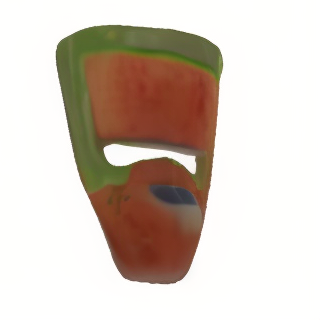
\includegraphics[width=\imgW]{images/comparison_plot/tiki_mask/zero123++unguided/avocado_couch_sdedit_steps_batch_0_tile_5.png} &
        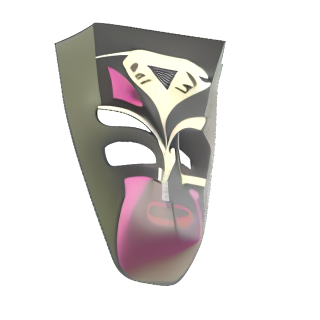
\includegraphics[width=\imgW]{images/comparison_plot/tiki_mask/zero123++guided/tiki_mask_guided_tile_5.png} &
        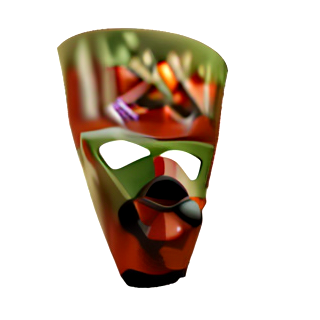
\includegraphics[width=\imgW]{images/comparison_plot/tiki_mask/zero123++refiner/split_image_2_5.png} &
        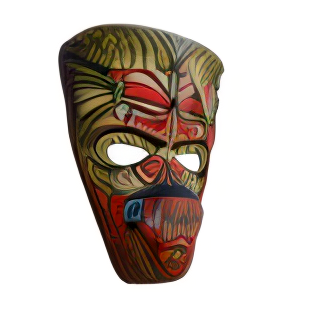
\includegraphics[width=\imgW]{images/comparison_plot/tiki_mask/sharp-e/10_75_steps_batch_0_a_wooden_tiki_mask_tile_5.png} \\
    \end{tabular}%
  }% end makebox

  \vspace{-12pt}
  \caption{%
    Comparison of Sharp-It with other methods for 3-D object enhancement.
    The first column shows the input generated by Shap-E; our method achieves
    the highest quality while best preserving the input.}
  \label{fig:mv2mv-comparisons}
\end{figure*}
\begin{table}[t]
    \caption{Quantitative comparison of our enhancement method with other baseline methods.}
    \vspace{-10pt}
    \label{tab:performance_comparison}
    \centering
    \setlength{\tabcolsep}{3pt} % Adjusts column padding for narrower width
    {\small % Keeps the font size at small
    \begin{tabular}{@{}lcccc@{}}
        \toprule
        \textbf{Method} & \textbf{FID $\downarrow$} & \textbf{CLIP $\uparrow$} & \textbf{DINO $\uparrow$} & \textbf{Runtime} \\ 
        \midrule
        GaussianDreamer & 50.89 & 0.81 & 0.82 &  6 min \\
        MVEdit & 44.87 & 0.83 & 0.77 &  1 min \\
        MVDream w/ SDEdit & 28.71 & 0.81 & 0.83 &  10 sec \\
        Zero123++ w/ SDEdit (U) & 24.59 & 0.87 & 0.86 &  10 sec \\
        Zero123++ w/ SDEdit (C) & 19.95 & 0.85 & 0.87 &  10 sec \\
        Zero123++ w/ SDEdit (R) & 19.13 & 0.87 & 0.89 &  10 sec \\
        Sharp-It & \textbf{6.60} & \textbf{0.90} & \textbf{0.92} &  10 sec \\
        \bottomrule
    \end{tabular}
    }
    \vspace{-12pt}
\end{table}

\begin{figure*}[t]
  %--- zero-width box that is shifted slightly left ---%
  \makebox[0pt][l]{\hspace*{\shift}%

    %------------- actual content -------------%
    \setlength{\tabcolsep}{3pt}
    \scriptsize
    \begin{tabular}{ccccccccc}
        & Input (Shap-E) & GaussianDreamer & MVEdit & MVDream w/ &
          Zero123++ w/ & Zero123++ w/ & Zero123++ w/ & Ours (Sharp-It)\\
        &                &                &         & SDEdit &
          SDEdit (U) & SDEdit (C) & SDEdit (R) \\[2pt]

        % avocado couch ---------------------------------------------------- %
        \raisebox{43pt}{\multirow{2}{*}{%
          \rotlabel{``An avocado shaped\\leather couch''}}} &
        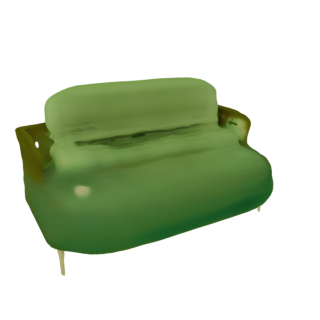
\includegraphics[width=\imgW]{images/comparison_plot/avocado_couch/shap-e/avocado_couch_view1_shap_e.png} &
        \includegraphics[width=\imgW,trim=30 30 30 30,clip]{images/comparison_plot/avocado_couch/gaussian_dreamer/1.png} &
        \includegraphics[width=\imgW]{images/comparison_plot/avocado_couch/mvedit/1.png} &
        \includegraphics[width=\imgW]{images/comparison_plot/avocado_couch/mvdream/avo_couch_upscaled_3.jpg} &
        \includegraphics[width=\imgW]{images/comparison_plot/avocado_couch/zero123++/avo_couch_tile_2_3.jpg} &
        \includegraphics[width=\imgW]{images/comparison_plot/avocado_couch/zero123++image/avo_couch_tile_1_3.jpg} &
        \includegraphics[width=\imgW]{images/comparison_plot/avocado_couch/zero123++refiner/split_image_0_2.png} &
        \includegraphics[width=\imgW]{images/comparison_plot/avocado_couch/sharp-e/avocado_couch_view1_sharp_e.png} \\

        & % second couch row
        \includegraphics[width=\imgW]{images/comparison_plot/avocado_couch/shap-e/avocado_couch_view2_shap_e.png} &
        \includegraphics[width=\imgW,trim=30 30 30 30,clip]{images/comparison_plot/avocado_couch/gaussian_dreamer/3.png} &
        \includegraphics[width=\imgW]{images/comparison_plot/avocado_couch/mvedit/2.png} &
        \includegraphics[width=\imgW]{images/comparison_plot/avocado_couch/mvdream/avo_couch_upscaled_1.jpg} &
        \includegraphics[width=\imgW]{images/comparison_plot/avocado_couch/zero123++/avo_couch_tile_2_6.jpg} &
        \includegraphics[width=\imgW]{images/comparison_plot/avocado_couch/zero123++image/avo_couch_tile_1_6.jpg} &
        \includegraphics[width=\imgW]{images/comparison_plot/avocado_couch/zero123++refiner/split_image_0_5.png} &
        \includegraphics[width=\imgW]{images/comparison_plot/avocado_couch/sharp-e/avocado_couch_view2_sharp_e.png} \\[2pt]

        % bust -------------------------------------------------------------- %
        \raisebox{36pt}{\multirow{2}{*}{%
          \rotlabel{``A bust of a man\\with a beard''}}} &
        \includegraphics[width=\imgW]{images/comparison_plot/bust/shap-e/tile_0.png} &
        \includegraphics[width=\imgW]{images/comparison_plot/bust/gaussian_dreamer/0.png} &
        \includegraphics[width=\imgW]{images/comparison_plot/bust/mvedit/1.png} &
        \includegraphics[width=\imgW]{images/comparison_plot/bust/mvdream/white_tile1.jpg} &
        \includegraphics[width=\imgW]{images/comparison_plot/bust/zero123++/efbb32609fd44a4f849015e875bc57a1_tile_1.png} &
        \includegraphics[width=\imgW]{images/comparison_plot/bust/zero123++img/efbb32609fd44a4f849015e875bc57a1_tile_1.png} &
        \includegraphics[width=\imgW]{images/comparison_plot/bust/zero123++refiner/split_image_1_0.png} &
        \includegraphics[width=\imgW]{images/comparison_plot/bust/sharp-e/efbb32609fd44a4f849015e875bc57a1_tile_1.png} \\

        & % second bust row
        \includegraphics[width=\imgW]{images/comparison_plot/bust/shap-e/tile_2.png} &
        \includegraphics[width=\imgW]{images/comparison_plot/bust/gaussian_dreamer/bust_gaussian_dreamer_2.png} &
        \includegraphics[width=\imgW]{images/comparison_plot/bust/mvedit/2.png} &
        \includegraphics[width=\imgW]{images/comparison_plot/bust/mvdream/white_tile2.png} &
        \includegraphics[width=\imgW]{images/comparison_plot/bust/zero123++/efbb32609fd44a4f849015e875bc57a1_tile_3.png} &
        \includegraphics[width=\imgW]{images/comparison_plot/bust/zero123++img/efbb32609fd44a4f849015e875bc57a1_tile_3.png} &
        \includegraphics[width=\imgW]{images/comparison_plot/bust/zero123++refiner/split_image_1_2.png} &
        \includegraphics[width=\imgW]{images/comparison_plot/bust/sharp-e/efbb32609fd44a4f849015e875bc57a1_tile_3.png} \\[2pt]

        % tiki mask --------------------------------------------------------- %
        \raisebox{25pt}{\multirow{2}{*}{%
          \rotlabel{``A wooden\\tiki mask''}}} &
        \includegraphics[width=\imgW]{images/comparison_plot/tiki_mask/shap-e/render_0000-4.jpg} &
        \includegraphics[width=\imgW]{images/comparison_plot/tiki_mask/gaussiandreamer/0.png} &
        \includegraphics[width=\imgW]{images/comparison_plot/tiki_mask/mvedit/render_0000-3.jpg} &
        \includegraphics[width=\imgW]{images/comparison_plot/tiki_mask/mvdream/tile_0.jpg} &
        \includegraphics[width=\imgW]{images/comparison_plot/tiki_mask/zero123++unguided/avocado_couch_sdedit_steps_batch_0_tile_0.png} &
        \includegraphics[width=\imgW]{images/comparison_plot/tiki_mask/zero123++guided/tiki_mask_guided_tile_0.png} &
        \includegraphics[width=\imgW]{images/comparison_plot/tiki_mask/zero123++refiner/split_image_2_0.png} &
        \includegraphics[width=\imgW]{images/comparison_plot/tiki_mask/sharp-e/10_75_steps_batch_0_a_wooden_tiki_mask_tile_0.png} \\

        & % second tiki row
        \includegraphics[width=\imgW]{images/comparison_plot/tiki_mask/shap-e/render_0005-2.jpg} &
        \includegraphics[width=\imgW]{images/comparison_plot/tiki_mask/gaussiandreamer/3.png} &
        \includegraphics[width=\imgW]{images/comparison_plot/tiki_mask/mvedit/render_0005.jpg} &
        \includegraphics[width=\imgW]{images/comparison_plot/tiki_mask/mvdream/tile_1-2.jpg} &
        \includegraphics[width=\imgW]{images/comparison_plot/tiki_mask/zero123++unguided/avocado_couch_sdedit_steps_batch_0_tile_5.png} &
        \includegraphics[width=\imgW]{images/comparison_plot/tiki_mask/zero123++guided/tiki_mask_guided_tile_5.png} &
        \includegraphics[width=\imgW]{images/comparison_plot/tiki_mask/zero123++refiner/split_image_2_5.png} &
        \includegraphics[width=\imgW]{images/comparison_plot/tiki_mask/sharp-e/10_75_steps_batch_0_a_wooden_tiki_mask_tile_5.png} \\
    \end{tabular}%
  }% end makebox

  \vspace{-12pt}
  \caption{%
    Comparison of Sharp-It with other methods for 3-D object enhancement.
    The first column shows the input generated by Shap-E; our method achieves
    the highest quality while best preserving the input.}
  \label{fig:mv2mv-comparisons}
\end{figure*}
\begin{table}[t]
    \caption{Quantitative comparison of our enhancement method with other baseline methods.}
    \vspace{-10pt}
    \label{tab:performance_comparison}
    \centering
    \setlength{\tabcolsep}{3pt} % Adjusts column padding for narrower width
    {\small % Keeps the font size at small
    \begin{tabular}{@{}lcccc@{}}
        \toprule
        \textbf{Method} & \textbf{FID $\downarrow$} & \textbf{CLIP $\uparrow$} & \textbf{DINO $\uparrow$} & \textbf{Runtime} \\ 
        \midrule
        GaussianDreamer & 50.89 & 0.81 & 0.82 &  6 min \\
        MVEdit & 44.87 & 0.83 & 0.77 &  1 min \\
        MVDream w/ SDEdit & 28.71 & 0.81 & 0.83 &  10 sec \\
        Zero123++ w/ SDEdit (U) & 24.59 & 0.87 & 0.86 &  10 sec \\
        Zero123++ w/ SDEdit (C) & 19.95 & 0.85 & 0.87 &  10 sec \\
        Zero123++ w/ SDEdit (R) & 19.13 & 0.87 & 0.89 &  10 sec \\
        Sharp-It & \textbf{6.60} & \textbf{0.90} & \textbf{0.92} &  10 sec \\
        \bottomrule
    \end{tabular}
    }
    \vspace{-12pt}
\end{table}

\section{Experiments}
In this section, we evaluate the performance of \ourname{} in enhancing 3D objects generated by Shap-E. We compare our method against several baselines, conduct ablation studies to analyze the impact of different components, and demonstrate applications in 3D generation and editing.

\subsection{Qualitative and Quantitative Comparison}


\paragraph{Baselines}

We compare \ourname{} with various enhancement baselines. First, we compare against an SDS-based approach that was used in Spice-E~\cite{sella2024spicee}. Specifically, we use GaussianDreamer~\cite{yi2024gaussiandreamerfastgenerationtext}, initializing Gaussian Splatting with Shap-E's shape output and optimizing it with a text-to-image model. 
To make refining the thousands of objects in our test set practical, we limit the optimization time to six minutes per object.
We also include MVEdit~\cite{mvedit2024}, a multi-view editing method that  refines coarse 3D shapes.

\vspace{-10pt}
Another set of baselines combines multi-view image generation with SDEdit~\cite{meng2022sdedit}. Here, we render Shap-E’s shape into a multi-view image set and apply simultaneous edits across views to ensure consistency. Using SDEdit with a strength of 0.4, we add noise to each multi-view image and denoise it. For multi-view generation, we use both MVDream~\cite{shi2024mvdream}, which is guided by a text prompt, and Zero123++~\cite{shi2023zero123singleimageconsistent}, which is conditioned on an image rather than text.
With Zero123++, we test three configurations:
(i) Zero123++ w/ SDEdit (R), where we apply SDXL Refiner model (default strength value)~\cite{podell2023sdxlimprovinglatentdiffusion} on the frontal view of the object, and use this edited view to guide SDEdit across the multi-view set, (ii) Zero123++ w/ SDEdit (C), where SDEdit with Stable Diffusion (strength 0.75) is applied on the object's frontal view which is used to guide the multi-view SDEdit; and (iii) Zero123++ w/ SDEdit (U), where no image condition is used.
 

\vspace{-10pt}
\paragraph{Dataset}
We conduct our quantitative experiments on our test set described in Section~\ref{sec:data}.
% a subset of Objaverse~\cite{deitke2023objaversexluniverse10m3d} that was held out during the training of \ourname. Each object in this subset is first encoded into Shap-E's latent space and then enhanced using each method. 
To demonstrate our method's generalization capability, we also present results on objects generated directly by Shap-E from text prompts.

\vspace{-12pt}
\paragraph{Metrics}
To assess enhancement performance, we evaluate the image quality produced by each method. Specifically, we compute the FID~\cite{parmar2021cleanfid, heusel2017gans} between the enhanced views and our test set. Additionally, we evaluate the semantic and visual similarity of the enhanced shape with the ground-truth using CLIP~\cite{radford2021learning} and DINO~\cite{caron2021emerging} image encoders.

\vspace{-12pt}
\paragraph{Results}
We present a qualitative comparison in Figure~\ref{fig:mv2mv-comparisons}. The avocado couch and the tiki mask were generated by Shap-E, while the bust is an encoded object from the test set. As shown, our method preserves the objects' coarse details while producing high-quality, detailed enhancements. In contrast, other methods diverge significantly from the original objects and yield less realistic results. For instance, our method accurately generates a leather-like texture, whereas other methods struggle to enhance the flat appearance of the Shap-E-generated couch.
Our approach also maintains color consistency with the input shapes. This is evident in the couch's back section, where brown and green tints are faithfully preserved, as well as in the bust and tiki mask. Our method generates significantly more fine details compared to other methods, particularly visible in the intricate features of the bust and the textural elements of the mask. 
Results for the objects lifted to 3D are provided in the supplementary materials.
% Additional lifted results for each method are provided in the supplementary materials.

Quantitative comparisons are shown in Table~\ref{tab:performance_comparison}. Our method achieves the lowest FID, confirming it produces the highest-quality results. Furthermore, our method shows the best alignment with the ground-truth object, as indicated by the CLIP and DINO similarity metrics, The runtime of our method is comparable to or faster than other methods.



\subsection{Ablation Studies}


\begin{figure}
    \centering
    \setlength{\tabcolsep}{1pt}
    {\small
    \begin{tabular}{ccccc}
        & Input & W/o text  & W/o diverse & Full method \\
        && prompt & lighting \\
        %
        \raisebox{35pt}{\rotatebox[origin=c]{90}{View 1}} &
        \multicolumn{1}{c}{\includegraphics[width=0.24\linewidth, trim=50 0 50 0, clip]{images/ablation_plot/shap_e/mv_0_image_tile_1.png}} &
        \includegraphics[width=0.24\linewidth, trim=50 0 50 0, clip]{images/ablation_plot/no_prompt/no_prompt_tile_1.png} &
        \includegraphics[width=0.24\linewidth, trim=50 0 50 0, clip]{images/ablation_plot/single_hdr/single_source_tile_1.png} &
        \includegraphics[width=0.24\linewidth, trim=50 0 50 0, clip]{images/ablation_plot/full/full_tile_1.png} \\
        %
        \raisebox{35pt}{\rotatebox[origin=c]{90}{View 2}} &
        \multicolumn{1}{c}{\includegraphics[width=0.24\linewidth, trim=50 0 50 0, clip]{images/ablation_plot/shap_e/mv_0_image_tile_2.png}} &
        \includegraphics[width=0.24\linewidth, trim=50 0 50 0, clip]{images/ablation_plot/no_prompt/no_prompt_tile_2.png} &
        \includegraphics[width=0.24\linewidth, trim=50 0 50 0, clip]{images/ablation_plot/single_hdr/single_source_tile_2.png} &
        \includegraphics[width=0.24\linewidth, trim=50 0 50 0, clip]{images/ablation_plot/full/full_tile_2.png} \\
        %
        \raisebox{35pt}{\rotatebox[origin=c]{90}{View 3}} &
        \multicolumn{1}{c}{\includegraphics[width=0.24\linewidth, trim=50 0 50 0, clip]{images/ablation_plot/shap_e/mv_0_image_tile_5.png}} &
        \includegraphics[width=0.24\linewidth, trim=50 0 50 0, clip]{images/ablation_plot/no_prompt/no_prompt_tile_5.png} &
        \includegraphics[width=0.24\linewidth, trim=50 0 50 0, clip]{images/ablation_plot/single_hdr/single_source_tile_5.png} &
        \includegraphics[width=0.24\linewidth, trim=50 0 50 0, clip]{images/ablation_plot/full/full_tile_5.png} \\
        %
        \multicolumn{5}{c}{``A knight in full plate armor''}
    \end{tabular}
    }
    \caption{Qualitative ablation study. The first column shows the degraded input object generated by Shap-E. Subsequent columns show the effects of removing specific components: omitting the text prompt leads to reduced texture detail, while excluding diverse lighting results in a flatter appearance with less realistic shading. The full model achieves the most refined and detailed result.}
    \label{fig:ablation}
\end{figure}


We conduct ablation studies to assess the contributions of different components in \ourname. 
First, we examine the importance of using an input text prompt, which is not utilized in Zero123++~\cite{shi2023zero123singleimageconsistent, xu2024instantmesh}, the model upon which we build.
Second, we explore the effect of constructing the dataset with diverse lighting conditions, rather than using a single type of lighting.
% Specifically, we examine the importance of using an input text prompt and the effect of constructing the dataset with diverse lighting conditions. 

For this analysis, we train our method without each component individually and present the results in Figure~\ref{fig:ablation}.
For computational efficiency, ablation models (including the full method one) were trained for 400,000 steps, fewer than in our main experiments.
\begin{table}[ht]
    \centering
    \caption{Quantitative results of our ablation study. All models were trained for 400,000 steps.}
    \label{tab:ablation}
    \begin{tabular}{@{}lcccc@{}} % Align columns to the left
        \toprule
        \textbf{Ablation} & \textbf{FID $\downarrow$} & \textbf{CLIP $\uparrow$} & \textbf{DINO $\uparrow$}  \\ 
        \midrule
            W/o text prompt & 9.91 & \textbf{0.91} &0.91&  \\
        W/o diverse lighting  & 9.16 & 0.89 & 0.91 &  \\
        Full method & \textbf{8.06} & 0.89 & 0.91 \\

        \bottomrule
    \end{tabular}
    \vspace{-16pt}
\end{table}

In the first column, we show a shape generated by Shap-E, which serves as input to the models in the subsequent rows. In the second column, we omit the text prompt, instead using an empty prompt. As shown, without a guiding text prompt, the results lack detail and fail to achieve a metallic appearance. In the third column, we construct the dataset with a single lighting condition, leading to a notable enhancement of the input shape but still lacking finer details. The last column displays results from our full model, which successfully achieves a metallic look and produces highly detailed shapes. Importantly, our results are consistent with the coarse details of the input shape. The lifted object of this example is included in the supplementary materials.
We also quantitatively evaluate each configuration using the metrics described in the previous section. Results are provided in Table~\ref{tab:ablation}. While all configurations are comparable aligned with the ground truth object, the full model achieves the highest image quality.


\begin{figure*}
\centering

\setlength{\tabcolsep}{1pt}
{\small
\begin{tabular}{c c c c c c c c c}
    & \multicolumn{2}{c}{``A Gundam''} & { } & \multicolumn{2}{c}{``A tank''} & { } & \multicolumn{2}{c}{``A glass and metal battle-axe''} \\
    %
    \raisebox{20pt}{\rotatebox[origin=c]{90}{Input}} &
    \includegraphics[width=0.13\linewidth]{images/generation_results/shap-e/gundam/gundam_tile_1.png} &
    \includegraphics[width=0.13\linewidth]{images/generation_results/zero123/gundam/gundam_solo.jpg} & { } & 
    \includegraphics[width=0.13\linewidth, trim=0 0 0 60, clip]{images/generation_results/shap-e/tank/tank_tile_2.png} &
    \includegraphics[width=0.13\linewidth, trim=0 50 0 150, clip]{images/generation_results/zero123/tank/tank_rem.jpg} & { } & 
    \includegraphics[width=0.13\linewidth]{images/generation_results/shap-e/glass_battle_axe/glass_battle_axe_tile_4.png} &
    \includegraphics[width=0.13\linewidth]{images/generation_results/zero123/glass_axe/glass_axe_14_rem.jpg}
    \\
    %
      \raisebox{20pt}{\rotatebox[origin=c]{90}{View 1}} &
    \includegraphics[width=0.13\linewidth]{images/generation_results/sharp-e/gundam/a_gundam_75_steps_batch_0_a_gundam_tile_2.png} &
    \includegraphics[width=0.13\linewidth]{images/generation_results/zero123/gundam/gundam_tile_0.jpg} & { } & 
    \includegraphics[width=0.13\linewidth, trim=20 50 20 50, clip]{images/generation_results/sharp-e/tank/a_battle_tank_75_steps_batch_0_a_battle_tank_tile_4.png} &
    \includegraphics[width=0.13\linewidth, trim=0 20 0 20, clip]{images/generation_results/zero123/tank/tank_tile_0.png} & { } & 
    \includegraphics[width=0.13\linewidth]{images/generation_results/sharp-e/axe/2_250_steps_batch_0_a_battle_axe_made_out_of_glass_tile_0.png} &
    \includegraphics[width=0.13\linewidth]{images/generation_results/zero123/glass_axe/glass_axe_14_tile_0.jpg}
    \\
    %
    \raisebox{20pt}{\rotatebox[origin=c]{90}{View 2}} &
    \includegraphics[width=0.13\linewidth]{images/generation_results/sharp-e/gundam/a_gundam_75_steps_batch_0_a_gundam_tile_1.png} &
    \includegraphics[width=0.13\linewidth]{images/generation_results/zero123/gundam/gundam_tile_1.jpg} & { } & 
    \includegraphics[width=0.13\linewidth, trim=0 0 0 60, clip]{images/generation_results/sharp-e/tank/a_battle_tank_75_steps_batch_0_a_battle_tank_tile_2.png} &
    \includegraphics[width=0.13\linewidth, trim=0 0 0 20, clip]{images/generation_results/zero123/tank/tank_tile_4.png} & { } & 
    \includegraphics[width=0.13\linewidth]{images/generation_results/sharp-e/axe/2_250_steps_batch_0_a_battle_axe_made_out_of_glass_tile_4.png} &
    \includegraphics[width=0.13\linewidth]{images/generation_results/zero123/glass_axe/glass_axe_14_tile_3.jpg} \\
    %
    & \multicolumn{1}{c}{Ours} & \multicolumn{1}{c}{Zero123++} & { } & \multicolumn{1}{c}{Ours} & \multicolumn{1}{c}{Zero123++} & { } & \multicolumn{1}{c}{Ours} & \multicolumn{1}{c}{Zero123++} \\
     
\end{tabular}
}
\vspace{-8pt}
\caption{
Text-to-MultiView qualitative results. Our method generates a multi-view set by creating a 3D object with Shap-E and refining it with \ourname. In contrast, Zero123++ first generates a single image with Stable Diffusion, then produces a multi-view set conditioned on that image. This approach leads to geometric artifacts, such as flatness (gundam) and the Janus problem (tank). Leveraging Shap-E's 3D knowledge, our method yields high-quality, coherent objects. Additional 3D renderings of these results are provided in the supplemental.
}
\vspace{-12pt}
\label{fig:text-to-3d}
\end{figure*}

\section{Applications}
We now demonstrate the various applications enabled by \ourname. Specifically, we show how \ourname{} bridges the quality gap between Shap-E and multi-view-based 3D generation methods, while supporting diverse 3D generative applications.


\vspace{-16pt}
\paragraph{Text-to-3D Generation}
As discussed in previous sections, a common approach for text-to-3D synthesis involves first generating a nearly consistent multi-view image set~\cite{shi2024mvdream, wang2023imagedream, shi2023zero123singleimageconsistent}, followed by a sparse-view 3D reconstruction method~\cite{xu2024instantmesh}. By combining Shap-E with \ourname, we achieve text-to-multi-view image synthesis, enabling a complete pipeline for 3D generation (Figure~\ref{fig:method}).
In Figure~\ref{fig:text-to-3d}, we compare text-to-multi-view results from Zero123++ and our method. Our method achieves results comparable to Zero123++ in terms of image quality, while demonstrating superior geometric details. The advantage of using Shap-E as a first stage is particularly evident in the tank and Gundam examples. The tank produced by Zero123++ suffers from a Janus problem, where wheels incorrectly appear on two adjacent sides. Moreover, Zero123++ generates a flat Gundam figure, lacking geometric details. These results demonstrate the effectiveness of our pipeline: using a 3D-aware model to generate a coarse 3D object, followed by refinement using an image diffusion model.


\vspace{-12pt}
\paragraph{3D Object Editing}

\begin{figure}
    \centering
    \setlength{\tabcolsep}{1pt}
    {\scriptsize
    \begin{tabular}{ccccc}
        %
        & \multicolumn{4}{c}{``A table lamp'' $\longrightarrow$ ``A golden table lamp''} \\
        %
        \raisebox{12pt}{\multirow{3}{*}{\rotatebox[origin=t]{90}{Shap-Editor}}} &
                \includegraphics[width=0.15\linewidth, trim=70 45 70 40, clip]
                % L B R T
{images/editings/shap-editor/lamps/original/render_0000.png} &
                       \includegraphics[width=0.15\linewidth, trim=70 45 70 40, clip]
{images/editings/shap-editor/lamps/shap_e/original_shap_e_tile_0.png} &
                        \includegraphics[width=0.15\linewidth, trim=70 45 70 40, clip]
{images/editings/shap-editor/lamps/edit1_shap_e/golden_shap_e_tile_0.png} &
                       \includegraphics[width=0.15\linewidth, trim=70 45 70 40, clip]
{images/editings/shap-editor/lamps/edit1_sharp_e/0_75_steps_batch_0_a_golden_table_lamp_tile_0.png} \\
        %
        %
        & \multicolumn{4}{c}{``A table lamp'' $\longrightarrow$ ``A santa table lamp''} \\
        %
         &
                       \includegraphics[width=0.15\linewidth, trim=70 45 70 40, clip]
{images/editings/shap-editor/lamps/original/render_0000.png} &
                      \includegraphics[width=0.15\linewidth, trim=70 45 70 40, clip]
{images/editings/shap-editor/lamps/shap_e/original_shap_e_tile_0.png} &
                    \includegraphics[width=0.15\linewidth, trim=70 45 70 40, clip]
{images/editings/shap-editor/lamps/edit2_shap_e/santa_0.png} &
                      \includegraphics[width=0.15\linewidth, trim=70 45 70 40, clip]
{images/editings/shap-editor/lamps/edit2_sharp_e/0_75_steps_batch_0_a_santa_table_lamp_tile_0.png} \\
        %
        %
        & \multicolumn{4}{c}{``A blue beetle car'' $\longrightarrow$ ``A torquoise beetle car''} \\
        %
                        % L B R T

        \raisebox{12pt}{\multirow{3}{*}{\rotatebox[origin=t]{90}{DDPM Inversion}}} &
    \includegraphics[width=0.22\linewidth, trim=30 60 15 85, clip]
{images/editings/ddpm_inv/original/render_0000.png} &
           \includegraphics[width=0.22\linewidth, trim=30 60 15 85, clip]{images/editings/ddpm_inv/shap_e/original_shap_e_tile_0.png} &
           \includegraphics[width=0.22\linewidth, trim=30 60 0 85, clip]{images/editings/ddpm_inv/edit1_shap_e/torquoise_shap_e_tile_0.png} &
           \includegraphics[width=0.22\linewidth, trim=30 60 0 85, clip]{images/editings/ddpm_inv/edit1_sharp_e/torquoise_beetle_car_75_steps_batch_0_a_matte_torquoise_beetle_car_tile_0.png} \\
        %
        %
         & \multicolumn{4}{c}{``A blue beetle car'' $\longrightarrow$ ``A blue SUV''} \\
        %
         &
             \includegraphics[width=0.22\linewidth, trim=30 60 15 85, clip]{images/editings/ddpm_inv/original/render_0000.png} &
            \includegraphics[width=0.22\linewidth, trim=30 60 15 85, clip]{images/editings/ddpm_inv/shap_e/original_shap_e_tile_0.png} &
           \includegraphics[width=0.22\linewidth, trim=30 60 0 85, clip]{images/editings/ddpm_inv/edit2_shap_e/mv_0_image_tile_0.png} &
               \includegraphics[width=0.22\linewidth, trim=30 60 0 85, clip]{images/editings/ddpm_inv/edit2_sharp_e/blue_suv_75_steps_batch_0_a_metalic_blue_suv_tile_0.png} \\
        %
        %
        & Input Shape & Encoded Shaped & Edit & + \ourname{}
    \end{tabular}
    }
    \vspace{-4pt}
    \caption{
    Our method enhances edits performed in Shap-E's space (rightmost column). We show editing results obtained with an existing editing method (Shap-Editor), and demonstrate that DDPM Inversion, originally developed for image diffusion models, works with Shap-E and can be integrated with \ourname{}.
    }
    \vspace{-16pt}
    \label{fig:edits}
\end{figure}
Shap-E provides a latent space in which semantic manipulation of 3D shapes can be performed while maintaining 3D consistency. Our method enhances these edited shapes to achieve high-quality objects. We demonstrate our method's application with two different editing techniques.
First, we use Shap-Editor~\cite{chen2023shapeditor}, which trains a model that takes a Shap-E latent code and a text instruction to produce a new latent code corresponding to the edited shape. While this method enables diverse and fast editing of 3D shapes, it is bounded by Shap-E's quality limitations. \ourname{} addresses this limitation by enhancing the results produced by Shap-Editor.
Second, inspired by diffusion-based editing methods for images, we apply a technique that enables shape editing with Shap-E. Specifically, we apply Edit-Friendly DDPM Inversion~\cite{huberman2024edit} with Shap-E instead of an image diffusion model.

Results for both methods are shown in Figure~\ref{fig:edits}. By combining \ourname{} with existing editing methods, we enable various types of high-quality 3D edits. These include changing an object's shape (demonstrated by transforming a car into an SUV), adding decorations (shown with the Christmas lamp), and modifying colors (as seen with the golden lamp and turquoise car).


\vspace{-16pt}
\paragraph{Appearance Editing} \label{sec:app-edit}
\ourname{} enables detailed control over the appearance of a degraded shape using text prompts. Specifically, at inference time, we can apply a different prompt from the one used during the generation of the Shap-E object, facilitating appearance editing that accurately preserves the original shape. Examples of this application are presented in Figures~\ref{fig:teaser} and \ref{fig:edits-appearance}.

% \begin{figure}
    \centering
    \setlength{\tabcolsep}{1pt}
    {\small
    \begin{tabular}{cccc}
        %
        \multicolumn{4}{c}{``Golden Jewelry Box'' $\longrightarrow$ ``Suede Leather Jewelry Box''} \\
        %
        \includegraphics[width=0.22\linewidth]{images/editings/appearance_edit/box/jewls_tile_0.png} &
        \includegraphics[width=0.22\linewidth]{images/editings/appearance_edit/box/jewls_tile_1.png} &
        \includegraphics[width=0.22\linewidth]{images/editings/appearance_edit/box/jewlery_jewlery_box_2_75_steps_batch_0_a_suede_leather_jewlry_box_tile_0.png} &
        \includegraphics[width=0.22\linewidth]{images/editings/appearance_edit/box/jewlery_jewlery_box_2_75_steps_batch_0_a_suede_leather_jewlry_box_tile_1.png} \\
        %
        \multicolumn{4}{c}{``Glass City Tower'' $\longrightarrow$ ``Wooden City Tower''} \\
        %
        \includegraphics[width=0.22\linewidth]{images/editings/appearance_edit/tower/glass_city_tower_tile_0.png} &
        \includegraphics[width=0.22\linewidth]{images/editings/appearance_edit/tower/glass_city_tower_tile_1.png} &
        \includegraphics[width=0.22\linewidth]{images/editings/appearance_edit/tower/glass_city_tower_2_75_steps_batch_0_a_wooden_city_tower_tile_0.png} &
        \includegraphics[width=0.22\linewidth]{images/editings/appearance_edit/tower/glass_city_tower_2_75_steps_batch_0_a_wooden_city_tower_tile_1.png} \\
        %
        \multicolumn{4}{c}{``Leather Chair'' $\longrightarrow$ ``Leopard Print Leather Chair''} \\
        %
        \includegraphics[width=0.22\linewidth]{images/editings/appearance_edit/chair/mv_0_image_tile_0.png} &
        \includegraphics[width=0.22\linewidth]{images/editings/appearance_edit/chair/mv_0_image_tile_1.png} &
        \includegraphics[width=0.22\linewidth]{images/editings/appearance_edit/chair/chair_test_2_75_steps_batch_0_a_leopard_print_leather_chair_tile_0.png} &
        \includegraphics[width=0.22\linewidth]{images/editings/appearance_edit/chair/chair_test_2_75_steps_batch_0_a_leopard_print_leather_chair_tile_1.png} \\
        %
        \multicolumn{2}{c}{Input} & \multicolumn{2}{c}{Appearance Edit}
    \end{tabular}
    }
    \vspace{-6pt}
    \caption{
    \ourname{} allows to edit the appearance of a Shap-E object by changing the prompt during the enhancement step. 
    }
    \vspace{-14pt}
    \label{fig:edits-appearance}
\end{figure}
\begin{figure}
    \centering
    \setlength{\tabcolsep}{1pt}
    {\small
    \begin{tabular}{cccc}
        %
        \multicolumn{4}{c}{``A red velvet chesterfield chair''} \\
        %
                \includegraphics[width=0.24\linewidth, trim=20 20 40 40, clip]{images/editings/spice-e/velvet_chair/guidance/chair_0000.jpg} &
                \includegraphics[width=0.24\linewidth, trim=40 40 60 60, clip]{images/editings/spice-e/velvet_chair/spice-e/shap-e_tile_0.png} &

                \includegraphics[width=0.24\linewidth, trim=60 60 100 90, clip]{images/editings/spice-e/velvet_chair/sds/1.png} &
                \includegraphics[width=0.24\linewidth, trim=40 40 60 60, clip]{images/editings/spice-e/velvet_chair/sharp-e/a_red_velvet_chair_2_75_steps_batch_0_a_chesterfield_light_red_velvet_chair_tile_0.png} \\
        %
                \includegraphics[width=0.24\linewidth, trim=40 50 40 60, clip]{images/editings/spice-e/velvet_chair/guidance/chair_0001.jpg} &
                \includegraphics[width=0.24\linewidth, trim=40 50 40 60, clip]{images/editings/spice-e/velvet_chair/spice-e/shap-e_tile_1.png} &
                \includegraphics[width=0.24\linewidth, trim=50 60 50 90, clip]{images/editings/spice-e/velvet_chair/sds/0.png} &
                \includegraphics[width=0.24\linewidth, trim=40 50 40 60, clip]{images/editings/spice-e/velvet_chair/sharp-e/a_red_velvet_chair_2_75_steps_batch_0_a_chesterfield_light_red_velvet_chair_tile_1.png} \\
                
        %
        \multicolumn{4}{c}{``A cargo spaceship''} \\
        %
                \includegraphics[width=0.24\linewidth, trim=60 60 20 50, clip]{images/editings/spice-e/space_ship/guidance/render_0002.jpg} &
                \includegraphics[width=0.24\linewidth, trim=60 60 20 50, clip]{images/editings/spice-e/space_ship/spice-e/spice-e_tile_2.png} &
                \includegraphics[width=0.24\linewidth, trim=60 60 20 105, clip]{images/editings/spice-e/space_ship/sds/2.png}  &
                \includegraphics[width=0.24\linewidth, trim=60 60 20 50, clip]{images/editings/spice-e/space_ship/sharp_e/sharp_e_tile_2.png} \\
                
        %
                \includegraphics[width=0.24\linewidth, trim=0 0 70 70, clip]{images/editings/spice-e/space_ship/guidance/render_0000-2.jpg} &
                \includegraphics[width=0.24\linewidth, trim=0 0 70 70, clip]{images/editings/spice-e/space_ship/spice-e/spice-e_tile_0.png} &
                \includegraphics[width=0.24\linewidth, trim=0 0 95 95, clip]{images/editings/spice-e/space_ship/sds/0.png}&
                \includegraphics[width=0.24\linewidth, trim=0 0 70 70, clip]{images/editings/spice-e/space_ship/sharp_e/sharp_e_tile_0.png}  \\
                
        %
        Abstract 3D  & Spice-E & w/ SDS & w/ \ourname \\
        Guidance & & refinement & refinement
    \end{tabular}
    }
    \vspace{-8pt}
    \caption{
    \ourname{} refines outputs generated by Spice-E, in a faster and more visually appealing way than an SDS-based refinement.
    }
    \vspace{-14pt}
    \label{fig:controlled-generation}
\end{figure}

\vspace{-14pt}
\paragraph{Controlled Generation}
Previous works have trained models that provide coarse geometric control over objects generated by Shap-E. Similar to Shap-E-based editing methods, such approaches are bounded by Shap-E's quality limitations. We demonstrate high-quality controlled 3D generation by applying our method to shapes generated with Spice-E~\cite{sella2024spicee}.
We show these results in Figure~\ref{fig:controlled-generation}. Our method significantly improves both object textures and fine geometric details. Notably, while Spice-E~\cite{sella2024spicee} uses an SDS-based approach as a refinement step, which impacts its runtime, our method achieves comparable or better results while running an order of magnitude faster.

% \begin{figure}
    \centering
    \setlength{\tabcolsep}{1pt}
    {\small
    \begin{tabular}{cccc}
        %
        \multicolumn{4}{c}{``A red velvet chesterfield chair''} \\
        %
                \includegraphics[width=0.24\linewidth, trim=20 20 40 40, clip]{images/editings/spice-e/velvet_chair/guidance/chair_0000.jpg} &
                \includegraphics[width=0.24\linewidth, trim=40 40 60 60, clip]{images/editings/spice-e/velvet_chair/spice-e/shap-e_tile_0.png} &

                \includegraphics[width=0.24\linewidth, trim=60 60 100 90, clip]{images/editings/spice-e/velvet_chair/sds/1.png} &
                \includegraphics[width=0.24\linewidth, trim=40 40 60 60, clip]{images/editings/spice-e/velvet_chair/sharp-e/a_red_velvet_chair_2_75_steps_batch_0_a_chesterfield_light_red_velvet_chair_tile_0.png} \\
        %
                \includegraphics[width=0.24\linewidth, trim=40 50 40 60, clip]{images/editings/spice-e/velvet_chair/guidance/chair_0001.jpg} &
                \includegraphics[width=0.24\linewidth, trim=40 50 40 60, clip]{images/editings/spice-e/velvet_chair/spice-e/shap-e_tile_1.png} &
                \includegraphics[width=0.24\linewidth, trim=50 60 50 90, clip]{images/editings/spice-e/velvet_chair/sds/0.png} &
                \includegraphics[width=0.24\linewidth, trim=40 50 40 60, clip]{images/editings/spice-e/velvet_chair/sharp-e/a_red_velvet_chair_2_75_steps_batch_0_a_chesterfield_light_red_velvet_chair_tile_1.png} \\
                
        %
        \multicolumn{4}{c}{``A cargo spaceship''} \\
        %
                \includegraphics[width=0.24\linewidth, trim=60 60 20 50, clip]{images/editings/spice-e/space_ship/guidance/render_0002.jpg} &
                \includegraphics[width=0.24\linewidth, trim=60 60 20 50, clip]{images/editings/spice-e/space_ship/spice-e/spice-e_tile_2.png} &
                \includegraphics[width=0.24\linewidth, trim=60 60 20 105, clip]{images/editings/spice-e/space_ship/sds/2.png}  &
                \includegraphics[width=0.24\linewidth, trim=60 60 20 50, clip]{images/editings/spice-e/space_ship/sharp_e/sharp_e_tile_2.png} \\
                
        %
                \includegraphics[width=0.24\linewidth, trim=0 0 70 70, clip]{images/editings/spice-e/space_ship/guidance/render_0000-2.jpg} &
                \includegraphics[width=0.24\linewidth, trim=0 0 70 70, clip]{images/editings/spice-e/space_ship/spice-e/spice-e_tile_0.png} &
                \includegraphics[width=0.24\linewidth, trim=0 0 95 95, clip]{images/editings/spice-e/space_ship/sds/0.png}&
                \includegraphics[width=0.24\linewidth, trim=0 0 70 70, clip]{images/editings/spice-e/space_ship/sharp_e/sharp_e_tile_0.png}  \\
                
        %
        Abstract 3D  & Spice-E & w/ SDS & w/ \ourname \\
        Guidance & & refinement & refinement
    \end{tabular}
    }
    \vspace{-8pt}
    \caption{
    \ourname{} refines outputs generated by Spice-E, in a faster and more visually appealing way than an SDS-based refinement.
    }
    \vspace{-14pt}
    \label{fig:controlled-generation}
\end{figure}
\begin{figure}
    \centering
    \setlength{\tabcolsep}{1pt}
    {\small
    \begin{tabular}{cccc}
        %
        \multicolumn{4}{c}{``Golden Jewelry Box'' $\longrightarrow$ ``Suede Leather Jewelry Box''} \\
        %
        \includegraphics[width=0.22\linewidth]{images/editings/appearance_edit/box/jewls_tile_0.png} &
        \includegraphics[width=0.22\linewidth]{images/editings/appearance_edit/box/jewls_tile_1.png} &
        \includegraphics[width=0.22\linewidth]{images/editings/appearance_edit/box/jewlery_jewlery_box_2_75_steps_batch_0_a_suede_leather_jewlry_box_tile_0.png} &
        \includegraphics[width=0.22\linewidth]{images/editings/appearance_edit/box/jewlery_jewlery_box_2_75_steps_batch_0_a_suede_leather_jewlry_box_tile_1.png} \\
        %
        \multicolumn{4}{c}{``Glass City Tower'' $\longrightarrow$ ``Wooden City Tower''} \\
        %
        \includegraphics[width=0.22\linewidth]{images/editings/appearance_edit/tower/glass_city_tower_tile_0.png} &
        \includegraphics[width=0.22\linewidth]{images/editings/appearance_edit/tower/glass_city_tower_tile_1.png} &
        \includegraphics[width=0.22\linewidth]{images/editings/appearance_edit/tower/glass_city_tower_2_75_steps_batch_0_a_wooden_city_tower_tile_0.png} &
        \includegraphics[width=0.22\linewidth]{images/editings/appearance_edit/tower/glass_city_tower_2_75_steps_batch_0_a_wooden_city_tower_tile_1.png} \\
        %
        \multicolumn{4}{c}{``Leather Chair'' $\longrightarrow$ ``Leopard Print Leather Chair''} \\
        %
        \includegraphics[width=0.22\linewidth]{images/editings/appearance_edit/chair/mv_0_image_tile_0.png} &
        \includegraphics[width=0.22\linewidth]{images/editings/appearance_edit/chair/mv_0_image_tile_1.png} &
        \includegraphics[width=0.22\linewidth]{images/editings/appearance_edit/chair/chair_test_2_75_steps_batch_0_a_leopard_print_leather_chair_tile_0.png} &
        \includegraphics[width=0.22\linewidth]{images/editings/appearance_edit/chair/chair_test_2_75_steps_batch_0_a_leopard_print_leather_chair_tile_1.png} \\
        %
        \multicolumn{2}{c}{Input} & \multicolumn{2}{c}{Appearance Edit}
    \end{tabular}
    }
    \vspace{-6pt}
    \caption{
    \ourname{} allows to edit the appearance of a Shap-E object by changing the prompt during the enhancement step. 
    }
    \vspace{-14pt}
    \label{fig:edits-appearance}
\end{figure}

\vspace{-3pt}
